\documentclass[12pt, twoside]{article}
\usepackage[letterpaper, margin=1in, headsep=0.5in]{geometry}
\usepackage[english]{babel}
\usepackage[utf8]{inputenc}
\usepackage{amsmath}
\usepackage{amsfonts}
\usepackage{amssymb}
\usepackage{tikz}
\usetikzlibrary{quotes, angles}
\usepackage{graphicx}
\usepackage{enumitem}
\usepackage{multicol}

\newif\ifmeta
\metatrue %print standards and topics tags

\title{Regents Geometry}
\author{Chris Huson}
\date{January 2022}

\usepackage{fancyhdr}
\pagestyle{fancy}
\fancyhf{}
\renewcommand{\headrulewidth}{0pt} % disable the underline of the header
\raggedbottom

\fancyhead[LE]{\thepage}
\fancyhead[RO]{\thepage \\ Name: \hspace{4cm} \,\\}
\fancyhead[LO]{BECA / Dr. Huson / Geometry 6 Trigonometry}

\begin{document}
\subsubsection*{6.9 Classwork: Solving triangles \hfill CCSS.HSG.SRT.C.8}
Write an equation expressing $\tan \theta$ as a ratio of \emph{opposite} over \emph{adjacent}, then solve for the missing length.
\begin{enumerate}
\item Given right $\triangle JKL$ with $\overline{JK} \perp \overline{KL}$, $JK=8$, $m\angle J=24^\circ$. Let $x$ be the length of the side opposite $\angle J$, $x=KL$.
    \begin{flushright}
        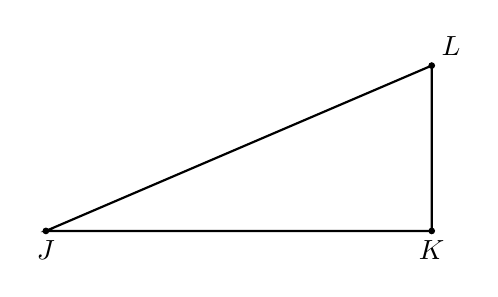
\begin{tikzpicture}[scale=0.7]
          \draw [thick](-1,0)--(6,0)--(6,3)--cycle;
          \draw [fill] (-1,0) circle [radius=0.05] node[below]{$J$};
          \draw [fill] (6,0) circle [radius=0.05] node[below]{$K$};
          \draw [fill] (6,3) circle [radius=0.05] node[above right]{$L$};
        \end{tikzpicture}
      \end{flushright} \vspace{3cm}

\item Given right $\triangle ABC$ with $m\angle C =90^\circ$, $BC=15$, $m\angle A=41^\circ$.
\begin{enumerate}
  \item Solve for $x=AC$.
  \item Find the length of the hypotenuse $AB$ using the Pythagorean theorem.
\end{enumerate}
  \begin{flushright}
      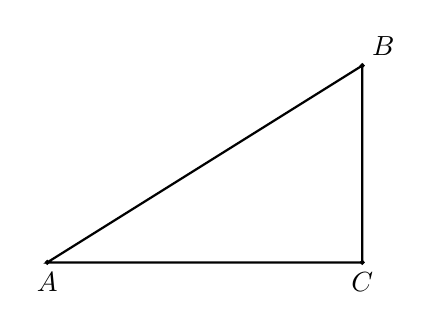
\begin{tikzpicture}[scale=0.5]
        \draw [thick](-1,0)--(7,0)--(7,5)--cycle;
        \draw [fill] (-1,0) circle [radius=0.05] node[below]{$A$};
        \draw [fill] (7,0) circle [radius=0.05] node[below]{$C$};
        \draw [fill] (7,5) circle [radius=0.05] node[above right]{$B$};
      \end{tikzpicture}
    \end{flushright}

\newpage
\item Given right $\triangle ABC$ with $m\angle C =90^\circ$, $BC=4$, $AC=19$, and $m\angle A=x^\circ$.
\begin{flushright}
  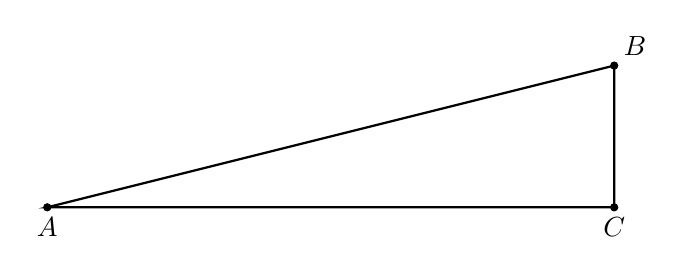
\begin{tikzpicture}[scale=0.9]
    \draw [thick](-1,0)--(7,0)--(7,2)--cycle;
    \draw [fill] (-1,0) circle [radius=0.05] node[below]{$A$};
    \draw [fill] (7,0) circle [radius=0.05] node[below]{$C$};
    \draw [fill] (7,2) circle [radius=0.05] node[above right]{$B$};
  \end{tikzpicture}
\end{flushright} \vspace{4cm}

\item Given right $\triangle ABC$ with $\overline{AC} \perp \overline{BC}$, $BC=7$, $m\angle B=55^\circ$. Let $x=AC$.
\begin{flushright}
  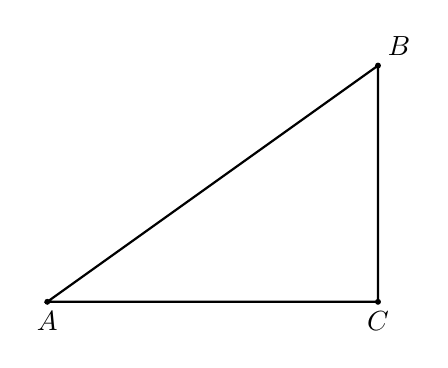
\begin{tikzpicture}[scale=0.6]
    \draw [thick](-1,0)--(6,0)--(6,5)--cycle;
    \draw [fill] (-1,0) circle [radius=0.05] node[below]{$A$};
    \draw [fill] (6,0) circle [radius=0.05] node[below]{$C$};
    \draw [fill] (6,5) circle [radius=0.05] node[above right]{$B$};
  \end{tikzpicture}
\end{flushright}

\newpage
\subsubsection*{Mastery topic: Algebraic solution}
\item Solve each equation for $x$, rounding to the nearest hundredth.
  \begin{enumerate}
  \begin{multicols}{2}
  \item $\displaystyle \tan 63^\circ = \frac{x}{14}$ \vspace{5cm}
  \item $\displaystyle \tan 77^\circ = \frac{10}{x}$
  \item $\displaystyle \tan 46^\circ  = \frac{x}{3.5}$ \vspace{5cm}
  \item $\displaystyle \tan 35^\circ = \frac{21}{x}$ 
  \end{multicols}
\end{enumerate}
  \vspace{6cm}
\item Solve for $x$, rounding to the nearest whole degree.
  \begin{enumerate}
  \begin{multicols}{2}
  \item $\displaystyle \theta = \tan^{-1} (\frac{12}{5})$ \vspace{4cm}
  \item $\displaystyle \tan \theta = \frac{3.2}{4.8}$ \vspace{4cm}
  \end{multicols}
\end{enumerate}

\newpage
\subsubsection*{Mastery topic: Calculator use}
  \item Express the result to the nearest thousandth. Angle measures are in radians. \vspace{.25cm}
    \begin{multicols}{2}
      \begin{enumerate}
        \item $\displaystyle \tan \frac{\pi}{4} = $ \vspace{1cm}
        \item $\displaystyle \tan \frac{\pi}{3} = $
        \item $\displaystyle \tan \frac{\pi}{6} = $ \vspace{1cm}
        \item $\displaystyle \tan \frac{\pi}{12} = $
      \end{enumerate}
    \end{multicols} \vspace{1cm}

  \item Find each value in radians, rounding to the nearest thousandths.\vspace{.25cm}
  \begin{multicols}{2}
    \begin{enumerate}
      \item $\tan^{-1} (1) = $ \vspace{1cm}
      \item $\tan^{-1} (\sqrt{3}) =$
    \end{enumerate}
  \end{multicols} \vspace{1cm}

  \item Convert between radians and degrees. Leave radians in terms of $\pi$.\vspace{.25cm}
  \begin{multicols}{2}
    \begin{enumerate}
      \item $45^\circ = $ \vspace{1cm}
      \item $\displaystyle \frac{\pi}{6} =$
    \end{enumerate}
  \end{multicols} \vspace{1cm}

  \item Round each value to the nearest hundredth. \vspace{.5cm}
  \begin{multicols}{2}
    \begin{enumerate}
      \item $AB=\sqrt{11^2+7^2}$ \vspace{3.5cm}
      \item $AB=\sqrt{3.2^2+1.9^2}$
      \item $AB=\sqrt{(-8.0)^2+(14.5)^2}$ \vspace{3.5cm}
      \item $AB=\sqrt{(4-3)^2+(7-11)^2}$
    \end{enumerate}
  \end{multicols} \vspace{1cm}

\end{enumerate}
\end{document}
